\documentclass{resume} % Use the custom resume.cls style

\usepackage[left=0.75in,top=0.6in,right=0.75in,bottom=0.6in]{geometry} % Document margins
\usepackage{xcolor}
\usepackage{graphicx}
\usepackage{newicktree}

\name{SampleName} % Your name
\address{Generated on \today} % Your address

\begin{document}
\textbf{Information on Clinical Annotation color coding}

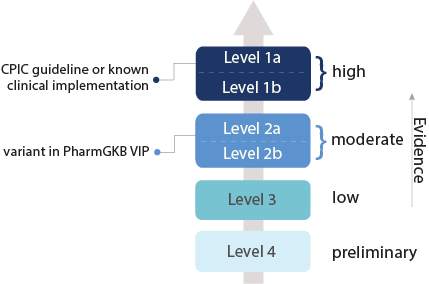
\includegraphics[scale=0.6]{levelsOfEvidence.png}

\begin{rSection}{Warfarin}
\item An anticoagulant that acts by inhibiting the synthesis of vitamin K-dependent coagulation factors. Warfarin is indicated for the prophylaxis and/or treatment of venous thrombosis and its extension, pulmonary embolism, and atrial fibrillation with embolization. It is also used as an adjunct in the prophylaxis of systemic embolism after myocardial infarction. Warfarin is also used as a rodenticide.

\begin{rSubsection}{VKORC1}{gene.geneDesc}{}{}
\item[]------------------------------------------------------ Dosing Guideline --------------------------------------------------------
\item \textbf{*1/*1} \newline Patients with the *1/*1 diplotype may require a higher dose of warfarin as compared to patients with the *2 or *3 CYP2C9 alleles. CYP2C9*1/*1 is considered a fully functional genotype. Other genetic and clinical factors may also influence a patient's required dose of warfarin 
\item[] ---------------------------------------------------- Clinical Annotations -----------------------------------------------------
\item \textbf{\colorbox{red}{Class 1A}} \textbf{rs1799853}  C/C \newline Patients with the CC genotype who are treated with warfarin may require a higher dose as compared to patients with the CT or TT genotype. Other genetic and clinical factors may also influence a patient's dose of warfarin.
\item  \textbf{\colorbox{orange}{Class 1B}} \textbf{rs1057910} A/A \newline Patients with the AA genotype: 1) may require an increased dose of warfarin as compared to patients with the AC or CC genotype 2) may have a decreased risk for adverse events as compared to patients with the AC or CC genotype. Patients with the AA genotype may still be at risk for adverse events when taking warfarin based on their genotype. Other genetic and clinical factors may also influence a patient's risk for adverse events.
\item  \textbf{\colorbox{yellow}{Class 2}} \textbf{rs7294} T/T \newline Patients with the TT genotype who are treated with warfarin may require a higher dose as compared to patients with the CC genotype. Other genetic and clinical factors may also influence a patient's required dose of warfarin.
\item  \textbf{\colorbox{green}{Class 4}} \textbf{rs9934438} G/G \newline Patients with the GG genotype who are treated with warfarin may require higher dose as compared to patients with the AG or AA genotype. Other genetic and clinical factors may also influence a patient's required dose of warfarin.
\end{rSubsection}

\end{rSection}

\end{document}